\title{Experience Report: Formalizing the DFUDS representation in Coq}

\author{Xuanrui (Ray) Qi}
\date{\today}

\documentclass[11pt]{article}

\usepackage{amsmath}
\usepackage{amssymb}
\usepackage{url}
\usepackage{hyperref}

\usepackage{graphicx}
\usepackage{subcaption}
\usepackage{layout}

\usepackage{minted}
\setminted{fontsize=\small}
\usemintedstyle{ssr}
\def\coqin#1{\mintinline{ssr}{#1}}

\usepackage{tikz}
\usetikzlibrary{calc,positioning,patterns,snakes}
\definecolor{coqgreen}{rgb}{0.1,0.8,0.0}

\begin{document}

\maketitle

\section{What is DFUDS?}
DFUDS, or \emph{depth-first unary degree sequence}, is a way to represent ordinal
trees (i.e., trees where the order of nodes matter) succinctly. The structure of
a tree of $n$ nodes can be represented in $2n + 2$, i.e., $O(n)$ bits maximum. This
is one of the most compact representations of ordinal trees besides the similarly
compact LOUDS (\emph{level-order unary degree sequence}) and BP (\emph{balanced parentheses})
representations, the former of which has been formalized in our previous work~\cite{succinct}). 

On a high level, DFUDS is very similar to LOUDS, except that DFUDS uses another traversal order:
LOUDS is based on level-order, i.e. breadth-first traversal, while DFUDS is based on pre-order
traversal. Each node is represented succinctly as a few bits in the resulting bit array. Our
algorithm is again based on~\cite{navarro}.

\newpage

\begin{figure}
\begin{subfigure}[t]{0.1\textwidth}
  \centering
  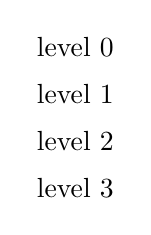
\begin{tikzpicture}[level distance=0.6cm,draw opacity=0,
    level 1/.style={sibling distance=1cm}]
    \node {level 0} 
      child { node {level 1} {
          child { node {level 2} {
            child { node {level 3} }
          } 
        }
      } } ;
  \end{tikzpicture}
\end{subfigure}
\begin{subfigure}[t]{0.44\textwidth}
  \centering
  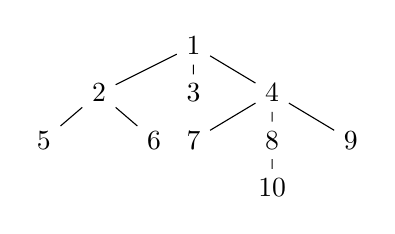
\begin{tikzpicture}[level distance=0.6cm,
    level 1/.style={sibling distance=1cm}]
    \node {1}
    child { node[xshift=-2mm]{2}
      child { node[xshift=-2mm]{5} }
      child { node[xshift=2mm]{6} } }
    child { node {3} }
    child { node {4}
      child { node {7} }
      child { node {8}
        child {node {10} } } 
      child { node {9} } } ;
  \end{tikzpicture} \\
  \caption{A sample tree}
  \label{fig:a_sample_tree}
\end{subfigure}
\begin{subfigure}[t]{0.44\textwidth}
  \centering
  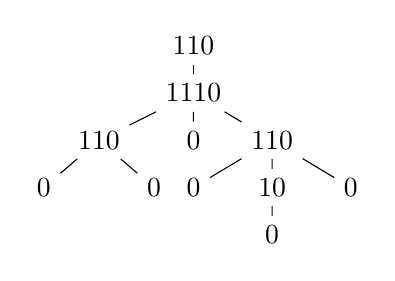
\begin{tikzpicture}[level distance=0.6cm,
    level 1/.style={sibling distance=1cm}]
    \node {110}
    child { node {1110}
      child { node[xshift=-2mm]{110}
        child { node[xshift=-2mm]{0} }
        child { node[xshift=2mm]{0} } }
      child { node {0} }
      child { node {110}
        child { node {0} }
        child { node {10}
          child {node {0} } } 
        child { node {0} } } } ;
  \end{tikzpicture} \\
  \caption{Its DFUDS vector encoding}
\end{subfigure}
\caption{DFUDS encoding of a sample unlabeled tree}
\label{fig:louds}
\end{figure}

One can see that DFUDS and LOUDS work very similarly on a high level: in fact, the node description
function used in both encodings are identical, and only the ``prefix'' is different. The substantial
difference between the two representations is thus in the traversal order.

In this brief work, we focused on formalizing just one DFUDS operation, $\mathbf{child}(B, v) =
\mathbf{succ_0}(B, v) - v$, where $B$ is the DFUDS encoding of a tree and $v$ is the position of a node
in the encoding.

\section{Take 1: direct implementation}
LOUDS use level-order traversal, which is tricky in functional programming, but DFUDS is just a structural
traversal over the tree, which we like. It is thus very easy to just implement DFUDS directly:

\begin{minted}{ssr}
  Definition describe_node (t : tree A) :=
    match t with
    | Node _ ch => rcons (nseq (size ch) true) false
    end.

  Fixpoint DFUDS' (t : tree A) :=
    match t with
    | Node _ ch => describe_node t ++ flatten [seq (DFUDS' t') | t' <- ch]
    end.

  Definition DFUDS t := [:: true; true; false] ++ DFUDS' t.
\end{minted}

This does not look too bad at all! However, it was a nightmare to prove using this directly implementation. We will
explain the reason very soon.

Defining position and the $\mathbf{children}(B, v)$ operation was not too hard, either:

\begin{minted}{ssr}
  Definition pred0 := pred false.
  Definition succ0 := succ false.

  Definition DFUDS_children B v := succ0 B v - v.

  Definition DFUDS_bits (t : tree A) := (number_of_nodes t).*2 - 1.
  
  Fixpoint DFUDS_position (t : tree A) (p : seq nat) := 3 +
    match t, p with
    | Node _ ch, [::] => 1
    | Node _ ch, h :: p' =>
      (size ch).+1 +
      sumn [seq (DFUDS_bits t') | t' <- take h ch] +
      DFUDS_position (nth t ch h) p'
    end.
\end{minted}

They do not look complicated, but proving anything about paths was a nightmare. The main problem is showing the relationship between
valid paths in the tree and the position in the DFUDS array.
When we are doing a level-order traversal, we descend one level at each step, corresponding perfectly
to one element in the ``path'', which is a array of indices of nodes at each level, so this was not a problem at all.

However, in DFUDS, this became a huge problem. Traversal does not really respect the path; when we descend into a path,
we must first fully traverse all preceding nodes. This makes it very painful. Therefore, even after profuse number of
attempts, I could not find a way to prove our main theorem in this direct implementation.

\section{Take 2: traversal with respect to a path}
We learn from the lessons of our previous work on LOUDS~\cite{succinct}, and first formalize tree traversal in the abstract. Moreover, we
describe an operation ``traversal up to a path'', which collects all nodes traversed when we follow a path. The standard pre-order traversal
is easy, and so is the proof about its size:

\begin{minted}{ssr}
  Fixpoint po_traversal_st (t : tree A) :=
    match t with
    | Node _ ch => (f t) :: flatten [seq (po_traversal_st t') | t' <- ch]
    end.

  Lemma po_traversal_st_size t : size (po_traversal_st t) = number_of_nodes t.
\end{minted}

It is easy to note that DFUDS is just specializing this function, flattening, and adding a prefix:

\begin{minted}{ssr}
  Definition DFUDS_st (t : tree A) := po_traversal_st describe_node t.
  
  Definition DFUDS (t : tree A) :=
    [:: true; true; false] ++ flatten (DFUDS_st t).
\end{minted}

That, however, is just generalizing our DFUDS operation a bit. What should we do about paths? The answer is that we can define another function
that corresponds to ``traversal up to a path''.

\begin{minted}{ssr}
  Fixpoint po_traversal_lt (t : tree A) (p : seq nat) :=
    let cl := children_of_node t in
    match p with
    | [::] => [::]
    | n :: p' =>
      f t ::
        flatten [seq (po_traversal_st f t') | t' <- take n cl] ++
        po_traversal_lt (nth t cl n) p'
    end.
\end{minted}

We collect all preceding nodes at each level and traverse them in full, and then traverse along the path. We can then show that it
is indeed correct by showing it collects all preceding nodes in pre-order. But first, we need a helper function defining the position
of a node in the pre-order traversal:

\begin{minted}{ssr}
  Fixpoint po_position (t : tree A) p :=
    let cl := children_of_node t in
    match p with
    | [::] => 0
    | n :: p' =>
      1 + sumn [ seq (number_of_nodes t') | t' <- take n cl ] +
      po_position (nth t cl n) p'
    end.

  Lemma po_traversal_lt_sizeE {B} (f : tree A -> B) (t : tree A) p :
    valid_position t p -> size (po_traversal_lt f t p) = po_position t p.  
\end{minted}

Then, we can express our desired correctness lemma. However, in the short time leading towards this project delivery, I was not able to
prove the lemma (the original LOUDS formalization took about a year!). It seems that we need to find a new proof technique for this, rather
than just induction on paths and trees:

\begin{minted}{ssr}
  Lemma po_traversal_ltE {B} (f : tree A -> B) (t : tree A) p :
    valid_position t p -> po_traversal_lt f t p = take (po_position t p)
                                                      (po_traversal_st f t).
\end{minted}

We also prove the ``mapping'' properties of pre-order traversal, as they will turn out to be useful since we often combine traversal with maps:

\begin{minted}{ssr}
  Lemma po_traversal_st_map {B : Type} (f : tree A -> B) (t : tree A) :
    po_traversal_st f t = map f (po_node_list t).
  
  Lemma map_po_traversal_st {B T} (f : tree A -> B) (g : B -> T) :
    map g \o [eta po_traversal_st f] =1 po_traversal_st (g \o f).
\end{minted}

We also have similar lemmas for \coqin{po_traversal_st}.

Then, the position of a nodes in DFUDS becomes just an instance of traversal up to a path (and then summing). For convenience we also define
DFUDS traversal up to a path, and prove that this traversal corresponds exactly to \coqin{DFUDS_position}:

\begin{minted}{ssr}
  Definition DFUDS_position t p :=
    let desc_l := po_traversal_lt description_length t p in
    4 + sumn desc_l.

  Definition DFUDS_lt (t : tree A) p := po_traversal_lt describe_node t p.
    
  Lemma DFUDS_positionE t p : valid_position t p ->
    DFUDS_position t p = 4 + size (flatten (DFUDS_lt t p)).
\end{minted}

The high-level definition of \coqin{DFUDS_children} and \coqin{DFUDS_childrenE} are the same as before, but the underlying internal implementation
is very different. The proof must proceed differently. In this short period of time, I was not able to complete the proof of
\coqin{DFUDS_childrenE} either, but I believe using the correspondences between traversal and traversal up-to a path, and more trial and
error, we can complete the proof. As far as I understand, most difficulties are purely engineering --- the expressions are very complicated.
However, we were able to prove some interesting small lemmas about DFUDS, such as the size of DFUDS:

\begin{minted}{ssr}
  Lemma DFUDS_sizeE t : size (DFUDS t) = (number_of_nodes t).*2.+2.
\end{minted}

I expect that if given a few months time \coqin{DFUDS_children} will not be a difficulty, but in such a short span of time, we simply do not have enough time
for enough trial-and-error.

\bibliographystyle{plain}
\bibliography{report}

\end{document}
